% Figure for 02_datasets.qmd, copied from slides/AE_week01_Intro/AE_w01_intro.tex.
% Compile with pdflatex, then convert: pdftocairo -svg <name>.pdf ../<name>.svg
\documentclass[class=extarticle, 9pt, tikz, border=4pt]{standalone}
\usepackage[T1]{fontenc}
\renewcommand{\familydefault}{\sfdefault}
\definecolor{PelloGrayDark}{RGB}{60,60,60}
\definecolor{PelloGray}{RGB}{120,120,120}
\definecolor{PelloGrayLight}{RGB}{235,235,235}
\definecolor{PelloGrayUltraLight}{RGB}{248,248,248}
\begin{document}
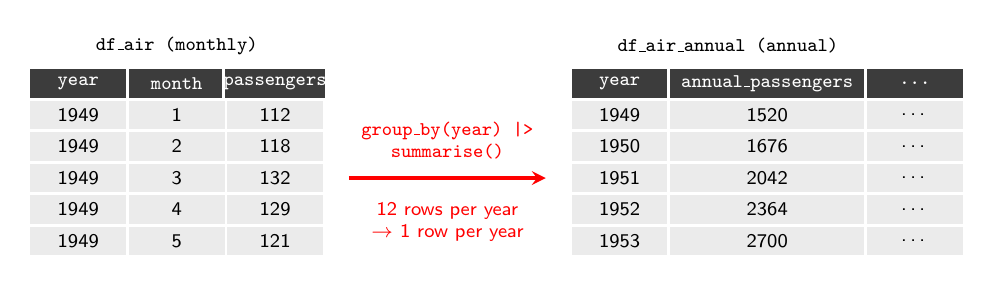
\begin{tikzpicture}[x=1.25cm, y=0.4cm, font=\scriptsize,
  cell/.style={draw=white, line width=1pt, fill=PelloGrayLight, minimum width=1.25cm, minimum height=0.4cm, inner sep=0pt},
  wide/.style={cell, minimum width=2.5cm},
  head/.style={fill=PelloGrayDark, text=white, font=\scriptsize\ttfamily}]
  % table titles
  \node[font=\scriptsize\ttfamily] at (1,1.2) {df\_air (monthly)};
  \node[font=\scriptsize\ttfamily] at (6.6,1.2) {df\_air\_annual (annual)};
  % headers
  \node[cell, head] at (0,0) {year};
  \node[cell, head] at (1,0) {month};
  \node[cell, head] at (2,0) {passengers};
  \node[cell, head] at (5.5,0) {year};
  \node[wide, head] at (7,0) {annual\_passengers};
  \node[cell, head] at (8.5,0) {\dots};
  % first five rows of each dataset
  \foreach \r/\v/\y/\s in {1/112/1949/1520, 2/118/1950/1676, 3/132/1951/2042, 4/129/1952/2364, 5/121/1953/2700} {
    \node[cell] at (0,-\r) {1949};
    \node[cell] at (1,-\r) {\r};
    \node[cell] at (2,-\r) {\v};
    \node[cell] at (5.5,-\r) {\y};
    \node[wide] at (7,-\r) {\s};
    \node[cell] at (8.5,-\r) {\dots};
  }
  % aggregation step
  \draw[red, line width=1.2pt, -stealth] (2.75,-3) -- (4.75,-3);
  \node[red, font=\scriptsize\ttfamily, align=center] at (3.75,-1.8) {group\_by(year) |>\\ summarise()};
  \node[red, align=center] at (3.75,-4.4) {12 rows per year\\ $\rightarrow$ 1 row per year};
\end{tikzpicture}
\end{document}
